%!TEX root = ../Thesis.tex
\chapter{Testing and Analysis}
The system mentioned in this work is complex and manual testing is not a viable approach, therefore automatic testing was implemented. For this purpose, an additional micro-service was introduced, called a performance test. It utilizes backend REST API to create reproducible test cases. It is also gathering the results and shows performance KPIs for the system. An example of test maps can be seen in appendix \ref{sec:app_04}.

\section{Test Cases}
The system was put through a series of tests using 14 different maps(examples in appendix \ref{sec:app_04}) of varying sizes and levels of complexity. Each algorithm being evaluated is run on each map, with the agents' positions remaining tests runs with different algorithms. End-to-end test time is measured, from when the calculation is triggered by the agent until the final path is determined. Additional information such as how long it took to set up the test, any communication time, and how long the algorithm took to calculate the path can be found in the observability suite \ref{sec:04_06_observability}. This allows for a thorough evaluation of the system's performance and helps identify any areas for improvement. Depending on the requirements, the system can be simulated in the cloud, run on an on-premises system, or even composed of virtual machines, those approaches are explained below. For the final test, an approach with the real on-premises system is used to examine communication delay to system performance.

\subsection{System simulated in the cloud}
The system can be simulated in a cloud-based environment. This is achieved by creating and connecting multiple agents to the system through the utilization of multiple Kubernetes pods spawned in a separate namespace. The simulation of the agent is performed in a cloud environment, and as such, this scenario does not take into account any communication delays as all containers are communicating within a local network (cluster network). This approach allows for the simulation of a cloud-based environment while maintaining control over the test conditions and minimizing external variables that may affect the results. This scenario is particularly useful for testing the system's scalability and performance under a cloud-based deployment.

\subsection{Real system}
A small-scale system composed of three external devices (Raspberry Pi) was constructed to demonstrate the functionality of a real-world system. On each of these devices, an agent container was deployed. One of the devices serves as the host for the map-service and broker containers. This configuration is shown in diagram \ref{fig:cluster}. This approach allows for the simulation of a real-world deployment scenario, while maintaining a manageable scale for testing and evaluation. This scenario is particularly useful for testing the system's functionality and performance under real-world conditions, as well as for evaluating the system's ability to integrate with external devices.

\begin{figure}[H]
    \centering
    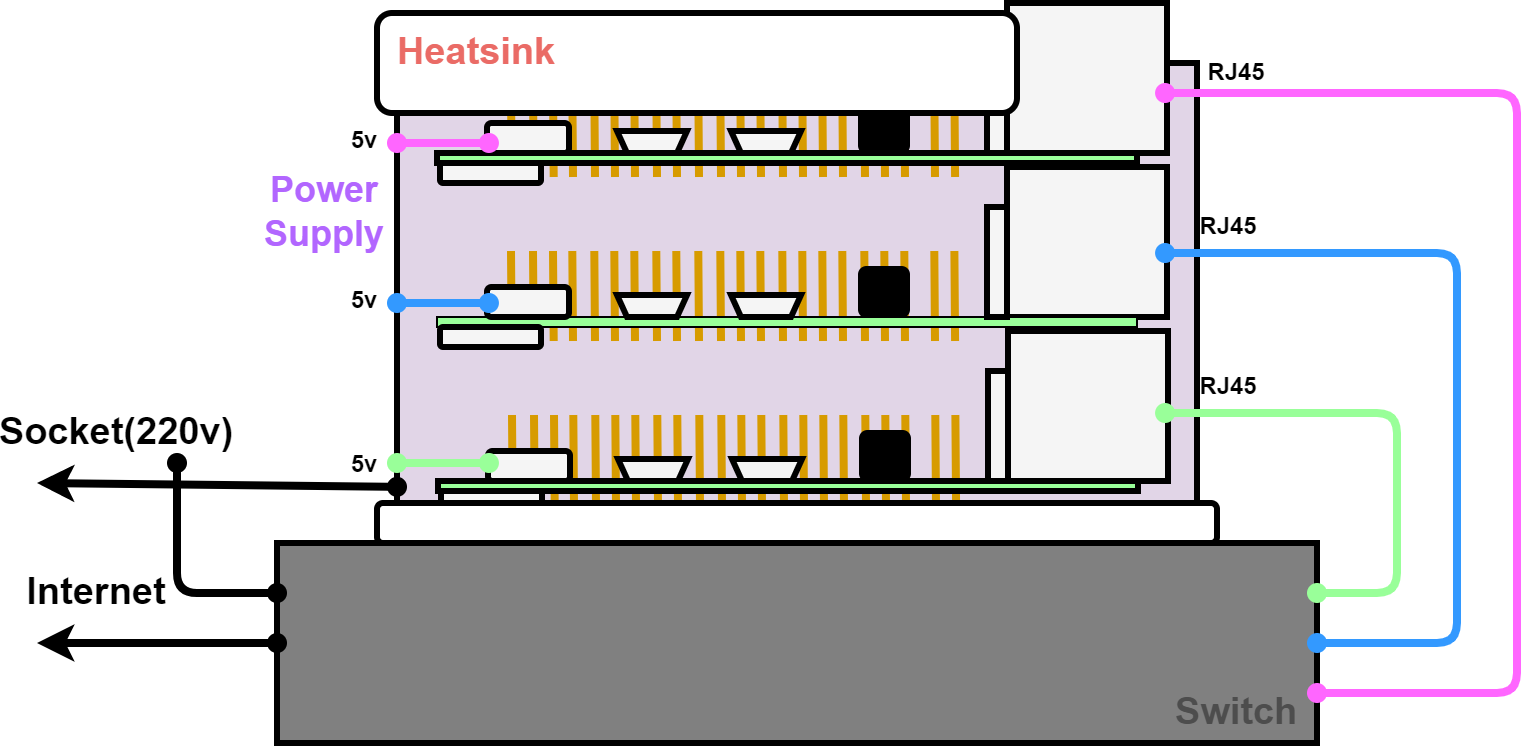
\includegraphics[width=0.8\textwidth]{pictures/cluster.png}
    \caption{ Real cluster }
    \label{fig:cluster}
\end{figure}

This setup resembles a real-world scenario, with 3 robots(agents) and one server meant for deploying brokers and communicating to the cloud. Agents have limited resources as Single Board Computer used for deployment only has 1GB of memory and Quad-core Cortex-A72 1.5GHz processor\cite{rpi_specs}. For the purpose of the test, computing power can also be throttled. Devices are connected to the local network via an internet switch. 

The challenging part was that those devices are using ARM architecture, therefore containers have to be rebuilt to support this architecture. To ease a development struggle, azure DevOps agents were installed on the machines and a Continous Integration pipeline was put in place, which rebuilds ARM images on every code change using local machines as hosts and pushes them into the image registry. The cloud part of the solution is deployed in okteto cloud and both parts are exchanging messages via MQTT brokers.

\subsection{System composed from virtual machines}
Another way of testing the system is to create a set of virtual machines or containers locally and connect them to the cloud system. The benefits of this approach are that this setup is easier to maintain, supports x86 architecture, and is easily extensible, as for spawning more agents there is no additional hardware needed. Resource limits can also be implemented both in the case of containers and virtual machines. Those entities have to be put in the same virtual network to enable communication between simulated machines.

\section{Communication time vs geological location of the cluster}
\begin{figure}[H]
    \centering
    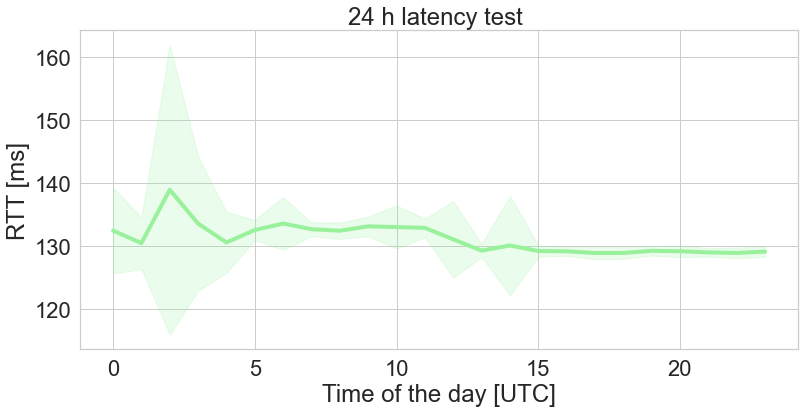
\includegraphics[width=0.8\textwidth]{pictures/ping.png}
    \caption{ RTT time }
    \label{fig:ping}
\end{figure}

\section{Comparison between computing time}
Test results for real agents were performed for agent devices forced to use half of their CPU and 512M of memory. Algorithms were grouped into a non-collaborative group(A*, Cloud A*) and a collaborative group(CA*, Cloud CA*), results can be seen in figures \ref{fig:on_prem_test_time} and in logarithmic scale on figure \ref{fig:on_prem_test_time_log}. The vertical axis represents the sum of paths computing time in milliseconds and the vertical axis indicates the dimension of the map i.ex map with dimension 5 will have 25(5x5) possible locations for the agent.

\begin{figure}
    \centering
    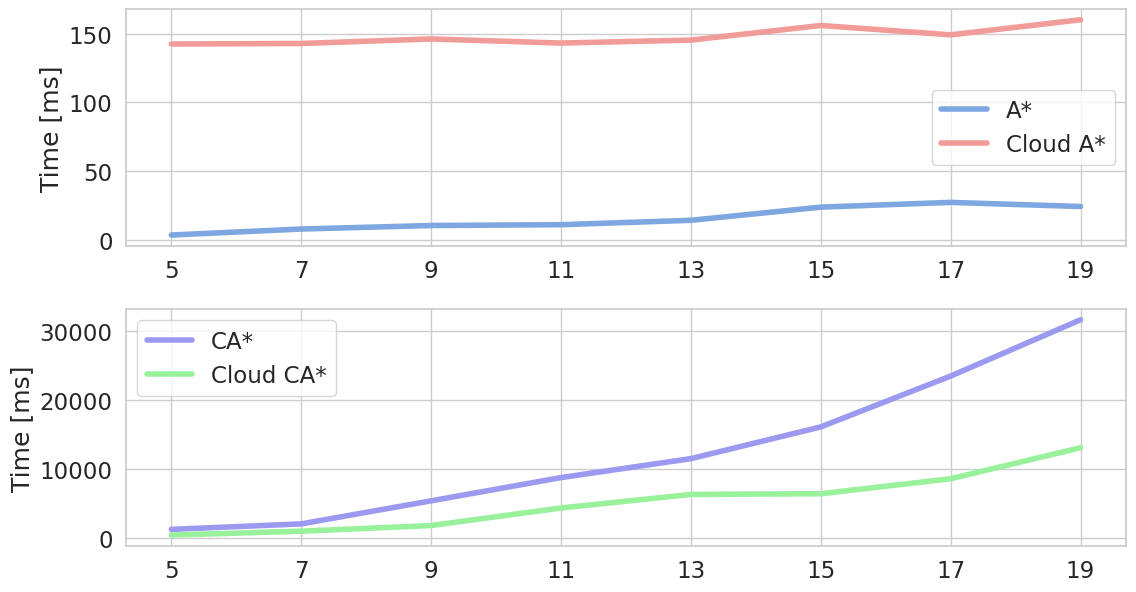
\includegraphics[width=0.75\textwidth]{pictures/on_prem_test_time.png}
    \caption{Test on on-prem setup}
    \label{fig:on_prem_test_time}
\end{figure}
\begin{figure}
    \centering
    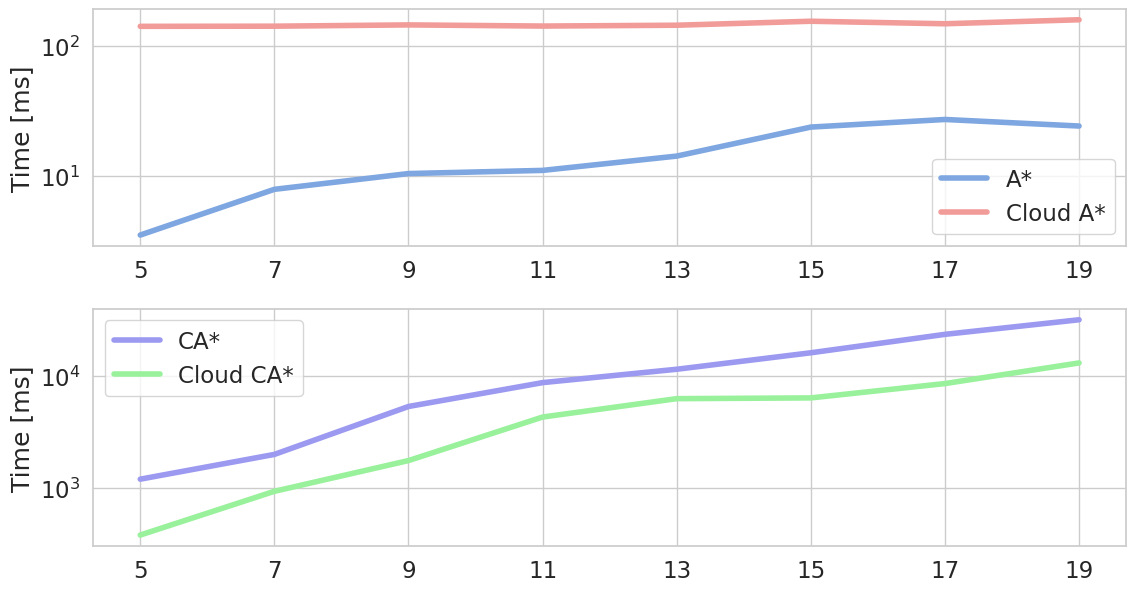
\includegraphics[width=0.75\textwidth]{pictures/on_prem_test_time_log.png}
    \caption{Test on on-prem setup in log scale}
    \label{fig:on_prem_test_time_log}
\end{figure}

The results of the performance testing indicate that non-collaborative algorithms are significantly faster than collaborative ones. The average time difference between A* and Cloud A* was found to be around 150ms, with A* being faster. Additionally, the results show that Cloud A* has a higher deviation than A*.

When comparing the results of CA* and Cloud CA*, it was found that CA* outperforms Cloud CA* on the smallest map. However, on larger maps, Cloud CA* performed better. The average performance of Cloud CA* was found to be around 10 times faster than CA*.

\section{Results by resources given to an agent}
\begin{figure}[H]
    \centering
    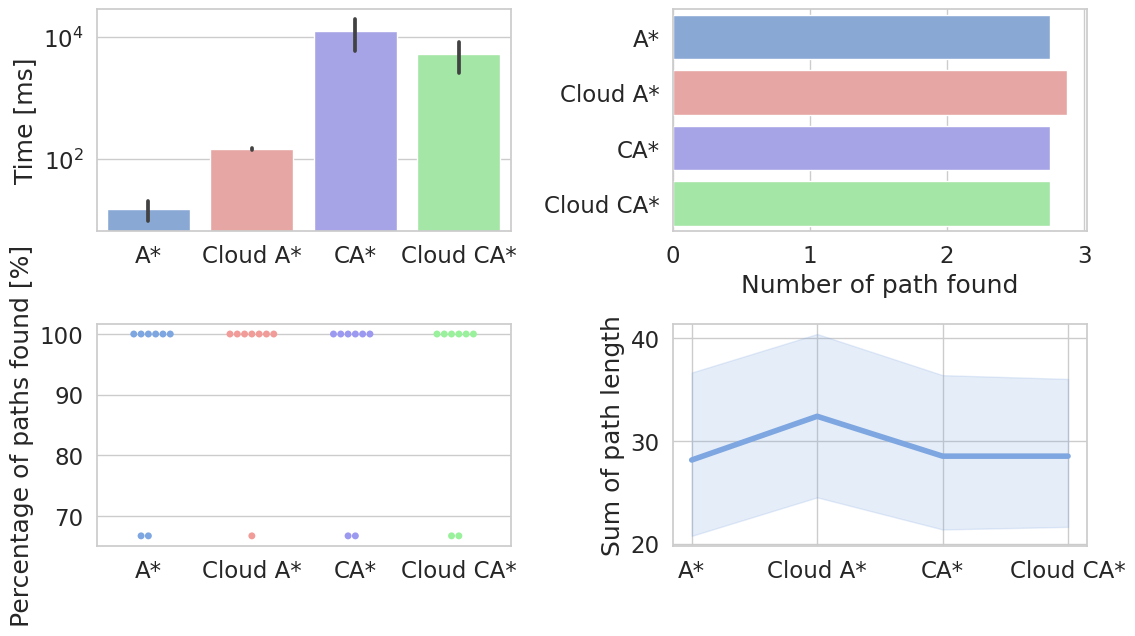
\includegraphics[width=0.8\textwidth]{pictures/on_prem_test_subplot.png}
    \caption{Test on on-prem setup}
    \label{fig:onprem_test_rest}
\end{figure}

